\documentclass[10pt, technote, draftcls, onecolumn]{IEEEtran}

%conference, compsocconf,

%\usepackage{pslatex} % -- times instead of computer modern

\usepackage{listings}
\usepackage{courier}


\usepackage{url}
\usepackage{booktabs}
\usepackage{graphicx}
%\usepackage{caption}
%\usepackage{subcaption}
\newcommand{\code}[1]{{\small{\textsf{#1}}}}
\newcommand{\codefoot}[1]{{\textsf{#1}}}
\usepackage{cite}
\usepackage{amsmath,amsthm}
\usepackage[usenames,dvipsnames]{xcolor}

\newcommand{\todo}[1]{{\emph{TODO: #1}}}

\usepackage{listings}
%\usepackage{subfigure}

% Packages for drawing state machines
\usepackage{pgf}
\usepackage{tikz}
\usetikzlibrary{arrows,automata}

\newcommand{\comment}[3]{\paragraph*{\textbf{#1}}{\color{#3}#2}}


\newcommand{\martin}[1]{\comment{Martin}{#1}{Blue}}
\newcommand{\david}[1]{\comment{David}{#1}{Blue}}
\newcommand{\cfelton}[1]{\comment{Chris}{#1}{Blue}}


\begin{document}

% MKL listings
\newcommand{\shdl} {
  \lstset{keywords={comp,end,def,in,out,if,then,else,true,false,
      int,real,bool,string,int1,int2,int3,int4,int5,int6,int7,int8,
      int16,int32,type}, 
    morecomment=[l]{//},
    morecomment=[s]{/*}{*/}, morestring=[b]{"},
    basicstyle=\ttfamily\small, showstringspaces=false,
    keywordstyle=\bfseries, mathescape=true, }}


%\title{Working title: Compare HDLs or\\
%Are New Hardware Description Languages Available for FPAG
%Development and Teaching Digital Design?}

\title{Are Modern Hardware Description Languages Ready for FPGA Design?}
\author{Martin Schoeberl\\
Department of Applied Mathematics and Computer Science, 
Technical University of Denmark\\masca@imm.dtu.dk
  \vspace{1ex}\\ 
David Broman\\
University of California, Berkeley and Link{\"o}ping University\\
broman@eecs.berkeley.edu
   \vspace{1ex}\\ 
Addition comments by Christohper L. Felton\\
cfelton@ieee.org
}



\maketitle \thispagestyle{empty}

\begin{abstract}
Since decades we use VHDL and Verilog as the main entry
languages for hardware design. Simulation and synthesize
tools support both languages quite well. Establishing a new
hardware description language and hoping for support from
the main tool vendors seems impossible.

However, in the last years several approaches for new hardware
description languages have been established. Those languages
provide advancements in software languages, such as dynamic
typing and object orientation, to the hardware designer.
The new languages usually provide their own frame work for
testing and simulation. However, for hardware synthesis they
use Verilog or VHDL as an intermediate language and therefore
have the full tool support.

In this paper we explore MyHDL, Chisel, and Bluspec for FPGA
design. We provide simple to medium complex designs in those
three languages and in VHDL as reference to show the different
features. From our experiments we conclude that all three languages
are ready to be used for new hardware designs.

\emph{an alternative abstract:}

Since decades we use VHDL and Verilog as the main entry
languages for hardware design. However, those are old languages
originally not designed for synthesize. In the mean time the software
community has made big improvements in programming languages
resulting in increased productivity.


%\cfelton{The above not designed for synthesis is not a useful
%point because an HDL needs to be a good language that describes the
%hardware and the synthesis flows from it.  That is why Verilog and VHDL
%have been successful with synthesis as well as modeling.  I don't
%believe any of the languages being reviewed have a complete bottom
%up synthesis oriented design?}

Can we leverage some of the development in programming
languages for hardware description? Several new hardware
description languages (HDL), based on software programming
languages, are proposed. In this paper we evaluate these
new HDLs and assess if they are ready for prime time.

\martin{Describe what we did find out}
\end{abstract}

\section{General}

Do some exploration of user base and available source code on all languages.

How many \emph{background} knowledge on programming language do we need for the new HDL?

Can it be a language to teach 1st and 2nd semester EE students to learn digital
electronics? Even without programming background? We now struggle with VHDL.

Languages to look at:

http://tomahawkins.org/ two languages at the bottom

\begin{itemize}
   \item MyHDL
   \item Chisel
   \item Lava
   \item Gezel
   \item JHDL
   \item Confluence
   \item HDCamel
\end{itemize}

\section{Introduction}

Verilog and VHDL has served us decades as the main languages for designing
digital systems. However, both languages have a large legacy and might not be
the most efficient languages to (1) build large digital systems and (2) to learn
hardware design.

In the software domain there has been a boom in new programming languages
in the last years. Programmers are more flexible now to change programming
languages when the job to been done is simplified. Within the hardware design
community a new HDL has a hard time to get established. As there is a way
smaller user base simulation and synthesize tools vendors are reluctant to
support a new HDL.

However, in recent year there have ben new approaches to use modern
languages as a basis for hardware design. The HDL is \emph{embedded}
in those new languages. The tool supporting this HDLs usually provide
support for simulation. For synthesize of hardware VHDL or Verilog is
generated. Therefore, the \emph{old} HDLs serve as an intermediate
language to have the full support of synthesize tools.

This paper compares modern hardware description languages and
assesses if they are mature and useful for FPGA designs.

The question is: is hardware design more productive with those new
languages? Are these languages mature enough for real world designs?
In this paper we explore several new HDLs in the context of hardware
design with FPGAs. When switching to a new design methodology one
wants to minimize risk and dependency on a a singe vendor. Open source
projects fulfill the role of risk minimization. In the worst case one can hire
someone to fix a bug in the HDL. Therefore, we restrict our language survey
to open-source projects.

\subsection{Assessment Criteria}


In synchronous design the two basic building blocks are combinational
(asynchronous) logic and flip-flop based registers. Larger on-chip
memories are not built out of registers, but are considered another building
block. This building blocks are also reflected in current FPGAs: lookup tables
(LUT) are used to implement combinational functions, dedicated flip-flops
the registers, on-chip memories support larger storage requirements,
and dedicated hard macros (with MAC operations) support efficient
implementation of DSP algorithms.

This results in following questions:
\begin{itemize}
\item Is it clear what is combinational logic and what are registers?
\item Can FPGA block RAMs be instantiated? Can ROMs be used?
\item Can the DSP blocks be used?
\end{itemize}

\todo{Write some text around the questions as motivation for them}

Further questions to be answered:

\begin{itemize}
\item Is simulation in the HDL possible?
\item Is there a clear line between the synthsizable  and not synthsizable parts of the language?
\item Can it be used in a first semester digital electronics course?
\item What about programming in the large? Are name spaces supported?
\item Quality of generated code: hardware resources and maximum clock frequency
\item Mixed language (with VHDL and/or Verilog) usage?
\item Size of the user group and support
\item Active development
\end{itemize}

Missing and hard to assess: productivity, easy to maintain.

\section{Getting Started}

This is a first tour through the languages.

\subsection{MyHDL}

Starting with MyHDL was a pleasure. Having Python already installed, the installation
of MyHDL was a matter of minutes. Having been exposed to Python for about one
day before, the first examples from the MyHDL manual~\cite{myhdl:2010} where easy as well.
However, jumping ahead and trying to generate some real VHDL code and programming
an FPGA with the HW version of \emph{Hello World} took some hours struggling
with cryptic error messages. The author is used to statically typed languages and
compile checks, where Pythons dynamic typing and interpreting execution model
reveals program and even typing errors only at runtime needs some adaption of
the authors programming mindset and habits.

The development approach in MyHDL is to test and verify the hardware within Python first
before generating VHDL or Verilog. Therefore, basic Python language knowledge is
needed for MyHDL. In fact MyHDL is less a language in its own, but a Python package.

\todo{Maybe this goes into a Discussion section at the end}

The question is if a dynamic typed language, where a variable can change the type
at runtime, the best base for HW synthesis is. In the resulting Verilog/VHDL code and
in the hardware the type of a signal or a register is statically fixed. Type errors in
Python are only detected at runtime by extensive testing. In a statically typed
language the compiler finds all type errors at compile time.

\cfelton{This is a common topic for dynamic languages like Python, strong typing
vs. dynamic typing.  Python has typing, you can't do $"me"+8$.  The subset of 
the HDL that explicitly describes the HDL to be converted has to be statically
typed.  The code is generated before ever running!  The types have be be defined.
You have this interesting mix of the embedded HDL.  As you pointed out, the converter
is not a compiler, it does not do (or intended) to do a thorough job of static 
analysis.  But the error messages are continuously improved by the myhdl community}

\todo{Comment: Python is easy going with dynamic typing and test benches run.
However, when converting to VHDL or Verilog, types (i.e., lengths of bit vectors)
need to be specified. As a result after high level simulation more work is needed
to have synthesizable code.}

\cfelton{Yes, myhdl is very similar to existing HDLs, the converter does close 
to a one-to-one translation from myhld to Verilog/VHDL.  But myhdl pushes the 
abstraction level as high as possible.  Example $intbv$ can be defined with 
$min$ and $max$ vs. the number of bits.  Long, time digital engineers we often
think in bits but when defining the $min$ and $max$ the intent is much clearer
for anyone else reading the code in the future!!!}

MyHDL takes a very software oriented approach to hardware design. The emphasis
is on unit test, which is a new a interesting approach in hardware design.
However, teaching digital electronic with VHDL showed the issues of students
thinking too much in the term of a \emph{program} instead of the hardware
structure. We think a HDL shall describe the actual structure and not an
algorithm in form of a software program.

\cfelton{software oriented \b{process} approach.  I totally disagree based on 
years of teaching HDL as well.  Students need to understand what a complex
digital system is and how the HDL works.  I have not run into many students
that do not quickly grasp the concurrent vs. sequential parts of the language.
How do you resolve this subjective point?  You would need a controlled study,
which is very difficult since digital hardware design is a small subset of 
Eng.  I do agree, highly concurrency vs. globally procedural needs to be 
emphasized when teaching new HDL'ers.  This is how many new languages are
evolving to support massive parallelism.}

\begin{itemize}
\item Very simple to download install
\item Python needs to be learned, some VHDL/Verilog knowledge is still needed
\end{itemize}

Installed on Python 2.7. Does it need a 2.x Python or would it run on 3.x as well?

\cfelton{it requires greater than 2.6 (for the 2.x versions).  Limited testing 
on 3.x.}

How large is the user base on MyHDL? Any open-source projects?

\cfelton{This is hard to gauge.  There are many users that come along and implement
a project or use for work.  But might not revisit for a couple years, the nature of 
their work.  They only implement new HDL every couple years.  Overall the active
user base is smallish, around a dozen or so}

see \url{http://thread.gmane.org/gmane.comp.python.myhdl/2701}

\subsubsection{Remarks}

Why does the manual show code for a simple mix that is not convertible to VHDL?

\cfelton{?? some pointers to these examples would be useful.  In the manual it
does differentiate between modeling (which the myhdl author and contributors think
is important) and conversion.  Modeling there are examples that are not intended
to be converted.  All intended conversion examples should convert.  Also see the 
"myhdl by example" wiki page on myhdl.org}

This is not the way we would like the process for synchronous logic:

\begin{verbatim}
FOO_HDL: process (clk, reset) is
begin
    if (reset = '1') then
        sig <= '0';
    elsif rising_edge(clk)or falling_edge(reset) then
        sig <= to_std_logic((not to_boolean(sig)));
    end if;
end process FOO_HDL;
\end{verbatim}

The MyHDL manual introduces too early, too many non-synthesizable constructs.
They might be good for test benches, but that should be stated more explicit.

\cfelton{The author and contributors of myhdl believe the modeling to be one
of the important features of myhdl.  Not only implementation (conversion).  Many
developers build models and do trade-off studies before ever implementing.  
Have a process to work through a design (vs. simply an implementation) the 
myhdl community believes is important and modeling is part of that.  This is
where it gets difficult in small examples.  Obviously, in small academic examples
modeling before had etc. 

The following is an example of creating a reference model first before moving
onto the implementation.
http://www.programmableplanet.com/author.asp?section_id=2438&doc_id=254265
}

Positive is conversion to VHDL and Verilog.

\subsection{Chisel}

Chisel is a HDL developed at the University of California, Berkeley~\cite{chisel:dac2012}.
Chisel is embedded in Scala.

As the language is a research vehicle and mainly used internally, getting
started just with the tutorial is harder than getting started with MyHDL.
Besides learning Chisel, some knowledge of Scala is needed. Furthermore,
the tool flow for Chisel is based on the build tool sbt, which itself needs to
be learned.

The tutorial for Chisel is already a complex set of exercises, solution, and
automation for building those exercises. In our opinion this starts with a
too steep learning course. Therefore, we have cut down the tutorial to
the minimum of a hardware \emph{Hello World} program: a blinking LED
on an FPGA board.\footnote{This Chisel Hello World introduction is
available as part of our HDL comparison code at:
\url{https://github.com/schoeberl/comphdl/tree/master/hello-chisel}}

\todo{The tutorial starts too complex.}

\martin{Are enums missing? Does the bit width always need to be known?}

\martin{Check if asynchronous or synchronous reset is used.}

\martin{Looks like synchronous reset is used. That's bad :-(}

\subsubsection{Issues, Questions}

The automatic inference of the correct bit length can lead to surprising
results. ``val r1 = Reg(resetVal = UFix(0, size))'' describes a register with
size bits, but the expression ``val r1 = Reg(UFix(0, size))'' results in a single
bit register.

\subsubsection{FlexPRET/Chisel Questions}

Why are the pipeline registers individual gals per filed? Why not a Bundle,
which could also be used for component IO?

\subsection{Lava}

Lava is a HDL based on Haskell~\cite{Lava:1998}. The first version described
is focused on verification and does not yet support description of sequential
hardware. \todo{Assume that this is all gone and there are some more papers.}

\martin{Looks like this Lava thing is tight with Xilinx. VHDL code generation
is also mentioned.}

\section{Language Assessments}

In this section we will assess which languages fulfill the criteria proposed in
the introduction and answer the questions.

\subsection{Is it clear what is combinational logic and what are registers?}

\todo{Check Verilog}

In VHDL there is no clear distinction between combinational logic, flip-flop
registers,  and memories in the language. Registers (and memories) are
inferred from \emph{code patterns}. Furthermore, small errors can result
in unintended latches generated in processes that are intended to be combinational.

MyHDL has no distinct types for register of memory. However, it uses annotations
(so called decorators in Python) to mark a function representing
combinational logic with \code{@always\_comb} and a function where the
output is stored in registers with \code{@always(clk.posedge)}. We consider
this as an enhancement related to VHDL/Verilog \todo{Check Verilog}.

\subsection{Documentation and Tutorials}

The MyHDL distribution contains a mental~\cite{myhdl:2010} that includes
a tutorial.

\subsection{Active Community}

It is important that a new language has a active developer group that is
able to fix errors and incorporate changes when new (FPGA) technology
becomes available. Furthermore, an active forum for the language users
is beneficial for getting started.

MyHDL is developed and maintained by Jan Decaluwe with the help of
Christopher Felton.  

\section{Notes (from iPad/Dropbox)}

MyHDL

Having min and max values that cannot be implemented so in HW is strange. I would prefer just signed/unsigned with a power of 2 range.

MyHDL is not a new language, but a python package. Python is the language. If a HW description is embedded in a full blown general purpose language with a lot of libraries, how easy is it to see the boundaries of what is synthesizable hardware, what is test benches, unit tests, and even generator code?

There is no indication is parameters are input or output signals.

Testing looks convenient with all the Python support.

Are signal records/structures possible?

A dynamic (scripting) language depends very much on unit tests. Even typos are only
discovered when the code is executed. Static typed languages (such as Java
and Scala) can catch quite a lot of bugs and typos during compilation.

General

Is tri state supported?

Shall I look into C based HDLs?

SystemC?

SystemVerilog

\section{Case Study}

\section{Sport Watch}
In this example we model the functionality of a modern sport
watch. A sport watch can be used to 
measure the time of a sport activity. Besides measuring time for the
whole activity, the watch should also be able to show lap times. The
purpose of this example is to create a small circuit that includes both
a data path and an FSM.

The system has two buttons that generate input signals. Button $B_1$
is used for starting and stopping the timer, whereas button $B_2$ is
used both for measuring a lap time and to reset the timer to zero. More
specifically, the watch can be modeled to have three states: $S$
(timer stopped), $R$ (timer is running), and $L$ (the timer is
running, but showing lap time). The following timed FSM illustrates
the behavior of the watch.\\


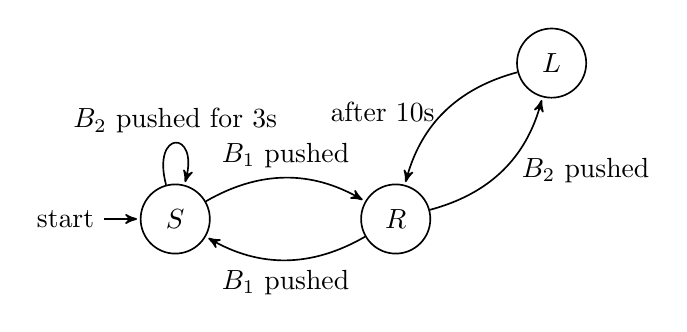
\begin{tikzpicture}[->,>=stealth',shorten >=1pt,auto,node distance=2.8cm,
                    semithick]
  \node[initial,state]                      (S) {$S$};
  \node[state]         [right of = S] (R) {$R$};
  \node[state]         [above right of = R] (L) {$L$};

  \path (S) edge [bend left]         node {$B_1$ pushed}        (R)
            edge [loop above]        node {$B_2$ pushed for 3s} (S)
        (R) edge [bend left]         node {$B_1$ pushed}        (S)
            edge [right, bend right] node {~$B_2$ pushed}       (L)
        (L) edge [left, bend right]  node {after 10s}           (R)
;
\end{tikzpicture}

Note that the loop edge at state $S$ resets the timer. The output
of the watch is a four digit display. When the watch is in state
$R$ and the elapsed time is below one minute, the display should show
seconds in the two most significant digits and fractions of seconds in
the two least significant digits. If the current time is more than one
minute, the two most significant digits show minutes and the least
significant digits seconds. When the state is in $L$, the display
should show the lap time, but the watch should continue to count in
the background.


\section{Further Notes and Reading Material}

MyHDL news group archive: \url{http://blog.gmane.org/gmane.comp.python.myhdl}


% \martin{This should not be in this paper:}
% \input{shdl}



\section{Conclusion}
\label{sec:conclusion}



\bibliographystyle{IEEEtran}
%\bibliographystyle{abbrv} % similar to IEEE without URLs
% pleas add bibs into other.bib as msbib.bib is 'generated'
\bibliography{msbib}

\section{Paper Plan}

Comparison to FPL 22 March

Extension of comparison to TII or TCAD

New language: Euromicro on DSD 11 March, ESWEEK 29 March, although best fit would be DAC and DATE

Embedded language without seeing the host: some program languages conference

\end{document}

